\documentclass[english,14pt]{beamer}
\usetheme{EastLansing}
\usecolortheme{spruce}

\usepackage{xcolor}
\usepackage{listings}
\usepackage{courier}
\usepackage{graphicx}
\usepackage{amsmath}
\usepackage{algorithm2e}
\usepackage{multicol}
\usepackage{hyperref}

% http://mirrors.ibiblio.org/CTAN/macros/latex/contrib/datetime2/datetime2.pdf
\usepackage{babel}
\usepackage[useregional]{datetime2}

% https://tex.stackexchange.com/questions/42619/x-mark-to-match-checkmark
\usepackage{pifont}% http://ctan.org/pkg/pifont

%% https://stackoverflow.com/questions/1435837/how-to-remove-footers-of-latex-beamer-templates
%%gets rid of bottom navigation bars
%\setbeamertemplate{footline}[page number]
%
%gets rid of navigation symbols
\setbeamertemplate{navigation symbols}{}


\usefonttheme[onlymath]{serif}

\definecolor{mGreen}{rgb}{0,0.6,0}
\definecolor{mGray}{rgb}{0.5,0.5,0.5}
\definecolor{mPurple}{rgb}{0.8,0,0.82}
\definecolor{backgroundColour}{rgb}{0.95,0.95,0.92}
\definecolor{lightBlue}{rgb}{0.1, 0.1, 0.8}

\newcommand\red[1]{{\color{red} #1}}
\newcommand\green[1]{{\color{green} #1}}
\newcommand\blue[1]{{\color{blue} #1}}

\newcommand{\cmark}{\ding{51}}%
\newcommand{\xmark}{\ding{55}}%

\lstdefinestyle{CStyle}{
    backgroundcolor=\color{backgroundColour},   
    commentstyle=\color{mGreen},
    keywordstyle=\color{magenta},
    numberstyle=\tiny\color{mGray},
    stringstyle=\color{mPurple},
    basicstyle=\footnotesize,
    breakatwhitespace=false,         
    breaklines=true,                 
    captionpos=b,                    
    keepspaces=true,                 
    numbers=left,                    
    numbersep=5pt,                  
    showspaces=false,                
    showstringspaces=false,
    showtabs=false,                  
    tabsize=2,
    language=Python
}

\lstdefinestyle{pseudo}{
        basicstyle=\ttfamily\footnotesize,
        keywordstyle=\color{lightBlue},
        morekeywords={BEGIN,END,IF,ELSE,ENDIF,ELSEIF,PRINT,WHILE,RETURN,ENDWHILE,DO,FOR,TO,IN,ENDFOR,BREAK,INPUT},
        morecomment=[l]{//},
        commentstyle=\color{mGreen}
}

\lstset{basicstyle=\footnotesize\ttfamily,breaklines=true}
\lstset{framextopmargin=50pt,tabsize=2}

\title{ENGG1003 - Thursday Week 4}
\subtitle{Using random numbers, and reading from spreadsheets}
\author{Steve Weller \& Sarah Johnson}
\institute{University of Newcastle}
%\date{\today}
\date{18 March, 2021}

% following is a bit of a hack, but forces page numbers (technically: frame numbers) to run 1,2,3,... 
% with titlepage counting as frame 1

\addtocounter{framenumber}{1}
\titlepage

\begin{document}

\begin{flushleft}
{\scriptsize Last compiled:~\DTMnow}
\vspace*{-5mm}
\end{flushleft}
\framebreak

%==============================================================

\begin{frame}[fragile]

\frametitle{Lecture overview}
\begin{enumerate}
	\item Using random numbers

	\item[]
	
	\item Reading from spreadsheets

\end{enumerate}

\end{frame}

%==============================================================

\begin{frame}[fragile]

\frametitle{$1)$ Using random numbers}

\begin{itemize}
	\item reminder and recap
	\item random integers
	\item random floats
\end{itemize}

\end{frame}

%==============================================================

\begin{frame}[fragile]

\frametitle{Random integers: simulating fair coin toss}

\textbf{Example 1}\\
\vspace*{5mm}
\begin{itemize}
	\item generate array of 0s and 1s length $N$
	\item 0=heads, 1=tails
	\item expected number of 0s (heads)?
\end{itemize}

\end{frame}

%==============================================================

\begin{frame}[fragile]

\frametitle{Coin toss simulation}

\begin{itemize}
	\item Python code for coin toss
	\item headsTails.py
	\item live demo
\end{itemize}

\end{frame}

%==============================================================

\begin{frame}[fragile]

\frametitle{Random floats: engineering tolerance}

\textbf{Example 2}\\
\vspace*{5mm}
\begin{itemize}
	\item simulate values in a range
	\item need engineering application---part manufactured within a tolerance, calculate fraction outside range
\end{itemize}

\end{frame}

%==============================================================

\begin{frame}[fragile]

\frametitle{Engineering tolerance simulation}

\begin{itemize}
	\item Python code for engineering tolerance
	\item live demo
\end{itemize}

\end{frame}

%==============================================================

\begin{frame}[fragile]

\frametitle{Random floats: simulate dartboard}

\textbf{Example 3}\\
\vspace*{5mm}
\begin{itemize}
	\item values in circle
	\item plot red inside, blue outside
\end{itemize}

\end{frame}

%==============================================================

\begin{frame}[fragile]

\frametitle{Dartboard simulation}

\begin{itemize}
	\item Python code for dartboard
	\item dartboard.py
	\item live demo
\end{itemize}

\end{frame}

%==============================================================

\begin{frame}[fragile]

\frametitle{Dartboard simulation}

\begin{itemize}
	\item dartboard red/blue simulation output plots
	\item N=100,1000,10K
\end{itemize}

\begin{figure}[ht]
	\centering
	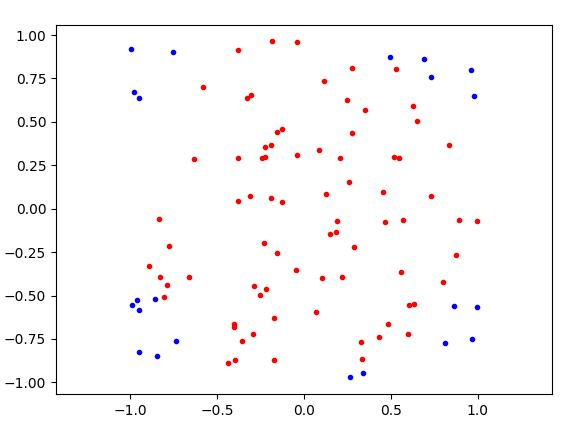
\includegraphics[width=0.3\textwidth]{figures/dartboard100}%
	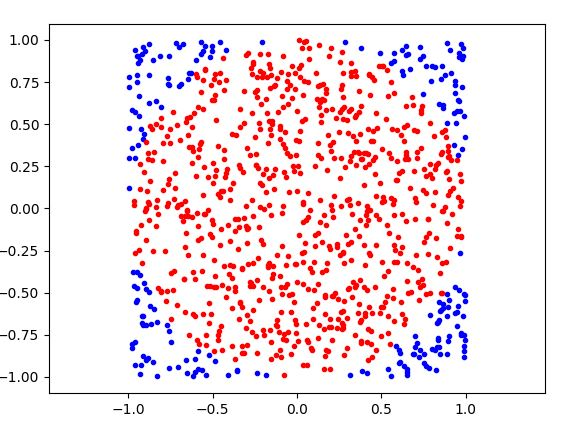
\includegraphics[width=0.3\textwidth]{figures/dartboard1000}%
	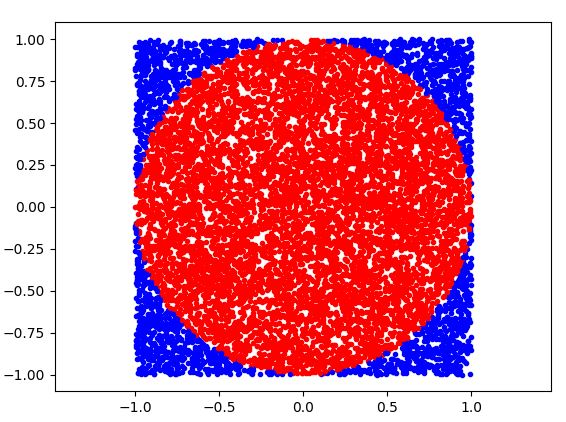
\includegraphics[width=0.3\textwidth]{figures/dartboard10000}
\end{figure}

\end{frame}

%==============================================================

\begin{frame}[fragile]

\frametitle{Random floats: estimate $\pi$}

\textbf{Example 4}\\
\vspace*{5mm}
\begin{itemize}
	\item modify previous example to count points inside circle, hence\ldots
	\item estimate $\pi$
\end{itemize}

\end{frame}

%%==============================================================
%
%\begin{frame}[fragile]
%
%\frametitle{}
%
%\begin{itemize}
%	\item xxx
%\end{itemize}
%
%\end{frame}
%
%%==============================================================
%
%\begin{frame}[fragile]
%
%\frametitle{}
%
%\begin{itemize}
%	\item xxx
%\end{itemize}
%
%\end{frame}
%
%%==============================================================
%
%\begin{frame}[fragile]
%
%\frametitle{}
%
%\begin{itemize}
%	\item xxx
%\end{itemize}
%
%\end{frame}

%==============================================================

\begin{frame}[fragile]

\frametitle{$2)$ Reading from spreadsheets}

%\begin{itemize}
%\item Lets see our code to calculate the height of a ball (from week 1) as a function
%\begin{lstlisting}[style=CStyle]
%# Function Definition
%def ball_height(v0, t):           # Function header
%    g = 9.81                     # Function body
%    y = v0*t - 0.5*g*t**2
%    return y                     # Return statement
%\end{lstlisting}
%\end{itemize}

\end{frame}

\end{document}